\documentclass[conference]{IEEEtran}
%\IEEEoverridecommandlockouts
% The preceding line is only needed to identify funding in the first footnote. If that is unneeded, please comment it out.
\usepackage{cite}
\usepackage{amsmath,amssymb,amsfonts}
\usepackage{algorithmic}
\usepackage{graphicx}
\usepackage{textcomp}
\usepackage{xcolor}
\def\BibTeX{{\rm B\kern-.05em{\sc i\kern-.025em b}\kern-.08em
    T\kern-.1667em\lower.7ex\hbox{E}\kern-.125emX}}
\begin{document}

\title{Social Media: A Social Engineers Goldmine\\
{\footnotesize \textsuperscript{}}
%\thanks{Identify applicable funding agency here. If none, delete this.}
}

\author{\IEEEauthorblockN{Henry Collier}
\IEEEauthorblockA{\textit{Computer Science} \\
\textit{College of Engineering and Applied Science}\\
\textit{University of Colorado, Colorado Springs}\\
W. Berlin, USA \\
hcollier@uccs.edu}

}
\maketitle

\begin{abstract}
Social media is a goldmine for a well-versed social engineer. People put their entire lives on one form of social media or another. For a social engineer, this is an avenue for success as the goldmine found within social media is very data rich.  Whether a social engineer is attempting to “connect” with a potential victim to get close to them in order to steal their identity, or if they are trying to gather enough information to perform a targeted attack the end game is supported in the same manner by the information that the end user posts without realizing the risk associated with their actions.  The purpose of this paper is to demonstrate that a person’s actions on social media puts them at risk to a variety of issues from identity theft to becoming a victim of a malicious threat actor.  
\end{abstract}

\begin{IEEEkeywords}
social engineering, social media,human factors, and susceptiblity
\end{IEEEkeywords}

\section{Introduction}
The problem of social engineering is not new.  In fact, social engineering has been around longer than computers have been.  However, how a social engineer conducts their method of attack has changed and with the ever increasing use of social media, the social engineers game has become one that is easy for them to play. In order to demonstrate how much of a problem social engineering has become, this paper will look at three separate, but connected components that make it easier for a social engineer to be successful. First we will review what social engineering is and how it is conducted, then we will look at social media and how this phenomenon has increased the success rate of social engineers and finally we will look at the human factors that make social media a social engineers goldmine.  How this paper is further classified into subgruops can be found below in figure 1.  To begin this journey, we need to first delve into the darkness and try to shine some light on the mystery called social engineering. 
\begin{figure}[htbp]
\centerline{\includegraphics[scale= .40]{classification.jpg}}
\caption{Classification model }
\label{fig}
\end{figure}
\section{Social Engineering}

Social engineering is as old as time and comes in many forms.  There are several famous examples of social engineers conducting their trade—Frank Abignale and Kevin Mitnick are probably two of the most famous.  Abignale was able to convince people that he was a pilot, a physician, a lawyer, and a teaching assistant. Kevin Mitnick on the other hand used social engineering and dumpster diving to gain access to the LA bus system and to breach several computer systems. Both were eventually arrested and spent several years in prison for their exploits. 

Although social engineering has been around for a really long time, research on social engineering during the early days of the Internet was fairly limited.  One of the earliest articles found during the literature review for this survey paper was from 1994. Tony Greening from the University of Sydney conducted a research experiment using a simulated large-scale social engineering scheme to see if it was possible to obtain student’s passwords\cite{Greening:1996:AYS:228292.228295}. In this early research study, Greening was able to show that there were several user activities that contributed to how easy it was for a social engineering scheme to work.  When we look at those factors identified by Greening in 1994, we can see that very little has changed since then regarding how today’s users are susceptible. One of the most significant of the factors identified is a “failure to recognize an attack.” Failing to recognize an attack is still one of the most predominant factors that makes an individual susceptible to a social engineering attack.  If an attacker can work to gain the trust of the user, then the social engineering attack has a much higher propensity for success. 
It is clear that social engineering has become the most successful form of attacking an organization’s network infrastructure.  With all of the advancements in technology, the threat actors have realized that what would normally take them months or even years to do can be completed in weeks, days or even minutes through a well-planned, targeted social engineering attack. By targeting the weakest link (aka the user), a threat actor increases their chances of success while reducing the amount of resources required and time spent to conduct the attack. 

In order to understand why social engineering is so effective, we need to take a deeper look at what social engineering really is. Social engineering, in its most basic essence, is the art of exploiting users to gain access to a system\cite{Krombholz:2013:SEA:2523514.2523596}.  How the social engineer exploits the user is the key to understanding social engineering. The social engineer works to manipulate the user into giving them information that they otherwise would not have given out or afford the social engineer access to a system that they otherwise would not have gotten access to. Modern day users of technology use a number of different services that help social engineers leverage sophisticated attacks\cite{Krombholz:2013:SEA:2523514.2523596}. In the paper Social Engineering Attacks on the Knowledge Worker Krombholz, Hobel, Huber and Weippl identify that there are five different types of social engineering attacks: physical approaches, social approaches, reverse social engineering, technical approaches and socio-technical approaches\cite{Krombholz:2013:SEA:2523514.2523596}. By identifying that there are these distinct approaches to social engineering, Krombohlz et al confirm that social engineering is a multifaceted problem that needs a multifaceted approach to protecting against it. 

Since the user is the most vulnerable part of any information system, social engineering is superior to most other forms of hacking and will allow access to the most secure system \cite{krombholz_hobel_huber_weippl_2015}. Social engineering attacks have been advancing at almost the speed of technology.  As technology changes, so do the methods of attack; unfortunately, countermeasures to social engineering do not advance at the same speed.  In fact, threat actors have been getting increasingly sophisticated and adept with developing and deploying their social engineering attacks\cite{conteh_schmick_2016}. Add to the dilemma of countermeasures not keeping up with the speed and ability of the social engineers to sophisticate their attacks is the fact that most cyber incidents are global in nature and law enforcement officials are limited by jurisdictional boundaries which makes prosecuting a social engineer even more difficult\cite{conteh_schmick_2016}. 

The problem of social engineering is bad enough when we look at it from the surface.  However, social engineering as we know it is really starting to change in a way that may sound very science fiction like. Up until now we only had to worry about a person trying to social engineer us, but that is beginning to change. With advancement in technology happening every day, especially in the areas of artificial intelligence and machine learning, researchers are starting to look at what automated social engineering attacks look like. Social-technical attacks are where a social engineer integrates the traditional social engineering techniques with technology.  One area that this is being shown as an effective approach is on social media sites.  Social engineers are starting to use technology to help develop context-aware spam where the social engineer uses a person's relationships with others to develop a more targeted attack; furthermore, the social engineers are also developing social-phishing attacks that use the user's interests against them[Huber]. Finally, social engineers are developing social bots to mimic the actions of a social engineer, but can target hundreds of users at a time \cite{Huber:2010:CAS:1866423.1866435}\cite{wagner}\cite{Postnikoff:2018:RSE:3173386.3176908}.   Gathering information from social media sites using automated tools significantly increases the speed at which a social engineering attack can be developed. 

There have been several attempts to identify better ways of developing defense mechanism against social engineering. There is little doubt that more needs to be done. It is clear to most that social engineering a person to steal their identity or compromise their bank account is bad enough, but we also need to understand that social engineering can be used to create more havoc and instability by compromising a nation's infrastructure, which could lead to a devastating effect on the nation's economy or set them up for being attacked \cite{Green:2015:ISE:2808705.2808717}.  In an attempt to reduce the effectiveness of social engineering, researchers are looking into ways of teaching users how to identify a social engineering attack before the attack is able to be successful.

Brent Wilson from George Fox University developed a mock social engineering attack built around a baiting experiment showed that his subjects, college age students, considered themselves very confident in identifying and stopping a social engineering attack, but this over confidence actually made them more vulnerable\cite{Wilson:2018:ICS:3280489.3280529}.  Wilson showed that even people who think they are too smart to become a victim of social engineer are susceptible and that the best way to defend against social engineering is to help people to think and behave differently\cite{Wilson:2018:ICS:3280489.3280529}.

In another situation, members of the United States Air Force Academy conducted a social engineering experiment during a computer vulnerability competition. The social engineers attempted to gather information from the participants in order to win the competition themselves. Although the social engineering team was able to gather a significant amount of data, they did not win the competition.  In the end, when surveyed, the participants that were socially engineered believed they were less likely to be socially engineered and only gave up information because they believed the social engineers were part of the event\cite{Kvedar:2010:UFS:1858583.1858595}.  The social engineers might not have won the competition, but they did win the trust of the targets which is an important part of conducting a social engineering attack.  Kevedar et al were very successful in step 2 (Developing Relationships) of the phases of social engineer as seen in figure 2. In order to successfully develop a relationship with your target, you must get the target to trust you, as did the social engineers in this experiment. 
\begin{figure}[htbp]
\centerline{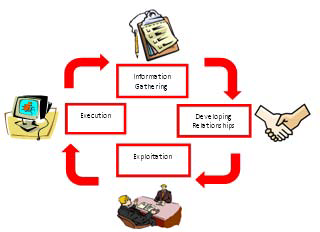
\includegraphics[scale= 1]{SocialEngineeringPhases.png}}
\caption{Social Engineering Phases \cite{Kvedar:2010:UFS:1858583.1858595}}
\label{fig}
\end{figure}
Omar Jaafor and Babiga Birregah from the University of Technology of Troyes took a different approach to trying to protect against social engineering by developing a multi-layered graph-based model for social engineering vulnerability assessment\cite{Jaafor:2015:MGM:2808797.2808899}.   Jaafor an Birregah argue that it is vital to conduct a vulnerability assessment of a system in relation to the system's vulnerability to social engineering. As part of their research, Jaafor and Birregah conducted several case studies and assessed the results.  In their conclusion, Jaafor and Birregah found that a multi-layered graph allowed them to capture the full diversity of channels and context an attacker uses to target and approach a victim\cite{Jaafor:2015:MGM:2808797.2808899}.  Furthermore, it was identified that the multi-layered graph was able to easily depict inter-connections between the channels\cite{Jaafor:2015:MGM:2808797.2808899}.  Understanding the underlying relationships between the channels and target vectors is important in trying to develop better mitigation strategies against social engineering. 

Organizations can employ individuals to conduct social engineering vulnerability testing, but need to understand the dynamics that are related to their employees if they do.  Conducting a physical penetration test that includes social engineering is both direct and personal which creates a level of risk that does not exist with other forms of vulnerability testing\cite{Dimkov:2010:TMP:1920261.1920319}.   Conducting a realistic vulnerably test that includes social engineering while not violating an employee's trust is going to be difficult, but it is possible. Dimkov et al conducted a couple of tests using two different formats and found that their environment-focused method was not only more reliable than their custodian-focused method, but also did not deceive the user as much and with the full back brief that was conducted, all stakeholders became aware of what was going on in a manner that was positive\cite{Dimkov:2010:TMP:1920261.1920319}.  

Ryan Heartfield and Geord Loukas of the University of Greewich go beyond most of the other researches in this field by further defining social engineering attack.  Heartfield and Loukas define the semantic attack as an attack that manipulates the user-computer interface to deceived the user and breach the security of the computer system\cite{Heartfield:2015:TAS:2856149.2835375}.   One of the things that Hearfield and Loukas identify is that the reason why semantic attacks are so difficult to defend against is the fact that most defenses are based on the attack signature and with semantic attacks, there is no definable signature that can be applied\cite{Heartfield:2015:TAS:2856149.2835375}. 

With the increased use of social media, a new series of social engineering attacks have been developed and have become exceedingly effective. Social engineers are targeting users of social media in ways that were not possible before the social media era.  For example, social engineers are creating fake profiles and using these profiles to target users, they are developing social phishing schemes and context-aware spam that has a higher success rate due to the “relationship” factor related to social media\cite{krombholz_hobel_huber_weippl_2015} With the increased use of cloud services and mobile applications people are connected to their data all of the time.  This 24hour/365-day connection, especially through social media, makes it more likely that a social engineer will be successful and gives them access to more data than previously could have been obtained through conventional methods.  

The addition of social media to the mix certainly exacerbates the problems associated with social engineering. While most of the damage done through social engineering via social media is personal in nature, a larger scale attack that targets multiple employees of an organization can have a significant impact to the organization\cite {Mills:2009:ASE:1940976.1941003}. The easiest and most consistent way for an attacker to gain entry into an organization is through an inside source.  These insiders who allow for an organization are also known as the non-malicious insider threat.  They are deemed non-malicious simply because they do not intend to harm the organization.   

Now that we understand how social engineering works and why it is so devastating, we need to look at how social media is feeding the fire realted to social engineering.  In the next section, we will take a deeper look a social media and what makes it a prime target space for social engineers. 
\section{Social Media}

\subsection{Usage}

No one can argue that social media has created an environment where old friends can connect, where friends and family that are separated by distance and time zones can remain connected and share all of life’s joys. With all of the great and wonderful uses that social networking sites were created to foster comes some serious concerns that most users do not fully realize. In the paper \textit{Undergraduate Student Perceptions of Personal Social Media Risk} by Rivera et al notes that “87\% of adults in the United States use the Internet” and that “in the 18-29 year old range, 89\% of Internet users us at least one form of social media\cite{Rivera:2015:USP:2885990.2885998}.”  Now if you take the number of users in the United States and then expand this number to include worldwide usage, the number of social media users becomes significant. The purpose of the paper by Rivera et al was to determine if undergraduate students understand the personal risks associated with social media. Rivera et al does not delve into the other age ranges in their research, but it is reasonable, and not a large leap of faith, to believe that the results from the undergraduate students group would follow suit to all users of social media. 

The results of the research conducted by Rivera et al showed the most undergraduate students do understand there is a threat associated with social media and that the most significant threat related to social media usage is identify theft\cite{Rivera:2015:USP:2885990.2885998}.  However, simply showing that undergraduate students perceive the risk of identity theft does not mean that they are better protected than someone who doesn’t perceive the threat.  Since most people do not take the most basic of security measure, like ensuring they only “friend” people that they actually know, or changing the security settings on their accounts to limit non-friends from accessing their information, they still put themselves at risk for being socially engineered and having their identities stolen. 

End user habits continually show that users of social media still put themselves in a position where a social engineer can obtain enough information to target them or steal their identity.  Although social media creates new avenues for social engineers to conduct their attacks, it must be noted that the threats associated with social media are not necessarily new. Weir, Tollan and Smeed evaluated the threats that exist within social media and determined that threats associated with social networking were simply “old wine in new bottles” in their paper \textit{The Threats of Social Networking: Old Wine in New Bottles}\cite{Weir:2011:TSN:2076032.2076216}. For example, the act of kidnapping someone is a physical crime that does not require the use of social networking. However, if the kidnappers might use social networking sites to conduct their reconnaissance and information gathering process which would both increase the amount of information they are able to obtain, but would also increase the speed by which the information was gathered.  Thus increasing the efficiency of their kidnapping plan and improving their chances of success.  Another real world example is that of home burglaries. Normally a thief would case the location, taking the chance of being spotted doing so. Now add social media into the mix where everyone loves to post pictures in real time while they are on vacation.  The thief can now find out that the homeowner is not at home without putting themselves at risk of being seen before the crime.  

Wu He from Old Dominion University notes in his paper \textit{A Review of Social Media Security Risks and Mitigation Techniques} that more than 50\% of his respondents reported an increase in malware due to their social media usage\cite{he_2012}.  To make things worse for the infected user, He continues on and shows that by breaching the trust of a single user and gaining access to their account, the attacker has the ability to pass along malware to the target user's ''friends''\cite{he_2012}.  This is very concerning because you are now not only at risk of putting yourself in jeopardy, but you are also subject to being victimized by your friends or putting your friends at risk. 

Kidnappers and thieves are not social engineers; however, they do deploy many of the same techniques as a social engineer would in conducting their illicit activities. More along the lines of a social engineer's work. Wier, Toolan and Smeed go on to show that it is possible for someone's social networking profile to lead to one of two forms of identity theft\cite{Weir:2011:TSN:2076032.2076216}. The first being true identity theft where the social engineer obtains enough information from the user's profile to actually steal the user's identity.  The second method is where the social engineer creates a fake profile and uses it to impersonate the targeted user\cite{Weir:2011:TSN:2076032.2076216}. Impersonating the target user can lead to many different outcomes, to include compromising different accounts, or perhaps targeting others that are “friends” of the target user.  

The picture is starting to look pretty clear, social media has become the perfect platform to deceive end users.  The reasons are pretty simple as to why and how. There is a perceived level of trust that social media users believe in, and with this perception they are setting themselves up to be deceived. In some cases, the deception occurs because the end user is naïve, but other times it is because the end user’s habits put themselves at risk. Placing too much personal information onto social media platforms puts the user at risk. 

Arun Vishwanath, from the University of Buffalo, conducted a research study to see if habitual use of Facebook had an impact on whether someone was able to be deceived on social media or not. During his research, Vishwanath worked to determine the susceptibility of a user to level 1 and level 2 phishing attacks. The level 1 phishing attack is also known as a stage 1 attack because this attack is often the first attack predicated by the attacker. The stage 1 attack is where the attacker works to make contact with the user by sending the user a friend request.  If accepted, a stage 2 attack is then conducted whereby the attacker sends a message that may include malicious links or malicious attachments\cite{doi:10.1111/jcc4.12100}.   The end results of Vishwanath’s study show that habitual Facebook use, where the user frequently uses Facebook and has a larger following, is the single largest predictor that a person may become victim to a social media attack\cite{doi:10.1111/jcc4.12100}.

Now let's step back a bit and take a broader look at social media and the risks associated with social media.  The threats to a user of social media are vast and the list is continuously growing. Phishers and spammers use social media to send fraudulent messages to users, social engineers and other cyber criminals use social media to capture end user's data that can then be used to create complex social engineering attacks on individuals\cite{ghari_shaabi_2012}. Add to this list of threats the sexual predators that use social media to target their prey and terrorists who use social media to try and broaden the impact of their terror attacks by developing propaganda and recruiting avenues\cite{ghari_shaabi_2012}. Let's not forget the nation state actors or political groups that use social media to try and sway political elections, as has been alleged for the 2016 US Presidential election\cite{ghari_shaabi_2012}. 

Social media creates a placed where a villain can do two very important things- steal and mislead\cite{Bernstein:2018:VGS:3209542.3210576} By working to mine online user's social media data, to include behavior, a threat actor can work to steal a person's identity, or develop a social engineering attack that can gain them access into the user's accounts and perhaps steal money from the user.  Furthermore, the threat actor can use social media to mislead users and work to manipulate them beyond gaining access to an account. In the article \textit{ A Villain’s Guide to Social Media and Web Science}, Bernstein and Hooper Identify that there are two distinct types of vulnerability- intrinsic and extrinsic. With the intrinsic vulnerability, the target is subject to attack through their circumstances and context, while with extrinsic vulnerability, the target is attacked due to the fact that they have some form of a secret that they wish to keep hidden\cite{Bernstein:2018:VGS:3209542.3210576}.  Identifying two different types of vulnerability is interesting in that doing so shows the complexity that exists in determining susceptibility and vulnerability.  The idea that if someone knows that certain behaviors put themselves at risk, does not mean that they will avoid those behaviors.  Rather, the human factor is so much more complex that this and trying to figure it out is not a simple process. 

There are many individuals who tout that they are privacy minded, yet their actions on social media contradict what they say.  A true privacy minded individual would either not answer certain questions when setting up their profile or answer incorrectly to shield the true information.  For example, when putting one’s birthdate into their social media account, a privacy minded person would obfuscate their real birthdate by changing the month/day or year.  For the person who wants to have their birthdate recognized and celebrated on social media, perhaps they put the real month/day, but choose a year that is different. Alas, the truth is astounding that many people answer with their true birthdate information.  

Ralph Gross and Alessandro Acquisti point out in their paper Information Revelation and Privacy in Online Social Networks that not only are the participation rates, especially among certain demographics, in online social networking usage astounding, but also the vast amounts and types of information freely revealed by the users is astonishing \cite{Gross:2005:IRP:1102199.1102214}. Gross and Acquisti do go on to show the complexity of the relationship between privacy and the user's social network by showing that it is very much multi-faceted\cite{Gross:2005:IRP:1102199.1102214}. Understanding that there is a difference between an “offline” social network and an “online” social network is important. Although the same type of information would be freely revealed in an offline social network, the negative impacts of such an event would be lessor than that of an online social network.   Most people have offline social networks, their friends, their families and their co-workers. How individuals interact in these offline social networks will often times follow on to their online social networks.  The biggest problem with this transfer of habits is the fact that in an online social network, the number of connections grows significantly. To add to this growth, you now have unknown or referred connections—the friends of your friends. 

Most of the “friends of your friends” problem can be addressed in most online social networks by simply ensuring your settings are correct.   Unfortunately, many social networking users either lack the knowledge of how to set up their accounts correctly or simply ignore these settings as unnecessary. The other issue with friends that are not really friends, but people who ask to be on your social media network, but don't actually know you.  This is another issue that can be addressed by appropriate usage techniques, but is often ignored.  After all, it is better to have online friends versus having only the 40 or 50 that you actually know. 

Historically speaking, social engineers were required to conduct their activities by interacting with the user.  With the advent of social media, social engineers were first able to simply become the users “friend” and then go to work on gathering information about the user that could be used against the user or to steal the user's identity. This manual process to obtain information to use in a social engineering attack is very time consuming. However, as Alim et al show in their research, automated methods of extracting data from social networking websites is quickly advancing and becoming more sophisticated and is the way forward for social engineers\cite{5402568}.   The research conducted by Alim et al was interesting in that they identified a few ways to advance the use of automated data extraction methods to go beyond the basic analysis of an end user. For starters, Alim et al identified that by using automated data extraction methods over a longer period of time the social engineer could monitor changes in the social network user profile, which could provide the social engineer with a deeper insight into their victim \cite{5402568}.  Additionally, Alim et al noted that automated data extraction methods could begin the process to target the others who have a connection to the first target \cite{5402568}.

Another technical method of attack is the “social bot.” The social bot is when an automated process is set up to mimic the actions of a real user\cite{wagner}. As machine learning and artificial intelligence continues to advance, the threat of a social engineering attack from a non-person grows.  If a social engineer can develop a social bot that targets hundreds of users at a time, then the social engineer receives a larger return on their investment. Similar to the concept of spam, where most spam is auto generated and sent, reducing the “cost” if sending hundereds upon hundreds of email, increases the return on the spammers investment every time someone falls prey to the spam. Wagner et al conducted research on the susceptibility of users to social bots and their results show that social users who were very active were more susceptible to social bot attacks\cite{wagner}.  The interesting part of their research is that the researchers had assumed that frequent users of social media would have developed skills that would help them identify a social bot attack over a legitimate user. However, the results showed that users don't develop those skills and with the advancements in machine learning and artificial intelligence, this is an alarming trend that is developing. 

So far we have looked at how social media usage can lead to a user being a victim of social engineered or simply being deceived by a threat actor.  Now let's look at two areas that people who are more security minded may not realize can create situations that help social engineers conduct their operations- information being leaked and information being inferred. 

\subsection{Leakage}

The threat of having one's information compromised due to a social engineer based on a person's social media usage is pretty significant. In fact, one might understand how easy it would be for a social engineer to attack them if their social media habits are not that secure. However, there is a threat that the user might not fully realize exists based on their social media usage, that threat is the leakage of their information.  When a user posts information to their social media account, they expect that information to be shared with their friends/family, but they don't expect that information to be shared with a third person that they are not directly linked to.  To compound this issue, a social media user's actions could lead to a compromise that does not directly impact the user themselves but perhaps others or their organization.  For example, a politician who posts about a secret trip to a foreign country not only puts the politician at risk, but also puts the entire security detail at risk, along with the success of the mission. Irresponsible use of social media leads to data leakage and data leakage opens the door to advanced persistent threats. An employee's social media habits, both intentional and unintentional, creates opportunities for the advanced persistent threats to realize their social engineering skills\cite{molok_chang_atif_ahmad_2010}. Candice Louw and Sebastiaan von Solms worked to develop a way to analyze the personally identifiably information that users share and with whom they share that data with\cite{Louw:2013:PII:2513456.2513467}. Preventing leakage may not be realistic, but perhaps understanding what data is leaked and how it is leaked will help reduce the impact of information leaked through social media.   

\subsection{Inference}

One area of concern regarding the risks associated with social media that isn't really looked at that much is the risk of an attacker inferring something about an individual based on their social media presence.  Through the application of neural networks and different machine learning algorithms, it is possible to infer sensitive, personal information about a user based on the insensitive public attributes of their social media profiles\cite{Mei:2017:IAB:3132465.3132469}.  Anytime sensitive personal information can be obtained about a person, the social engineer wins. As users, we need to work to prevent sensitive information from falling into the hands of those who would use it against us.  Inference attacks makes our job of protecting our data more difficult.  

Now that we understand social engineering better and how social media feeds into social engineering, we need to look deeper into the human factors that truly makes social media a goldmine for social engineers. 

\section{Human Factors}
\subsection{Susceptiblity}
In order to understand the human factors related to social media security, and what makes someone susceptible, it is important to understand how someone can be deceived on social media, but more simply to understand how someone can be deceived. In other words, what makes someone susceptible? 

Online deception is not much different than deceiving someone in person, the only difference is the medium in which the deception is processed. Deception is the favorite for gaining a strategic advantage\cite{Tsikerdekis:2014:ODS:2663191.2629612}. From the social engineer's perspective, deception is a tool that can be used to gain the trust of the target, which results in a successful social engineering attack. Social media creates an environment that makes deception easy because it is an environment that requires no assessment signals\cite{Tsikerdekis:2014:ODS:2663191.2629612}.  In addition to the lack of required assessment signals, there is the issue of trust that users afford the deceiver.  This trust given to the deceivers results in a reduction in suspicion by the user towards a deceiver, which ends in an increased likelihood of being deceived\cite{Tsikerdekis:2014:ODS:2663191.2629612}.  Some will argue that there are specific demographics that determine a person’s susceptibility to being deceived.  Sheng et al conducted a survey to see if they could determine the demographics that make someone more susceptible to phishing attempts\cite{Sheng:2010:FPD:1753326.1753383}.  What Sheng et al found out was that it was a person's technical knowledge and training level that was the true determining factor on a person's susceptibility and not a specific demographic trait, although initial results gave belive that women and younger people were more at risk\cite{Sheng:2010:FPD:1753326.1753383}. Sheng et al\cite{Sheng:2010:FPD:1753326.1753383}, Tsikerdekis and Zeadally\cite{Tsikerdekis:2014:ODS:2663191.2629612}, and Oehri and Teufel \cite{6320436} all believe that training and knowledge are the most useful tools to preventing the human factors from allowing a person to be deceived or become a victim of social engineering.  However, Robert Gibson states in his paper \textit{Who's Really in your Top 8: Network Security in the Age of Social Networking} that there really is no way to fully protect against a social engineering attack\cite{Gibson:2007:WRY:1294046.1294077}.  Yet as Gibson continues his paper, he notes that although there is no way to prevent an attack, it is quite possible to reduce the effectiveness of an attack. 

However, Frumento et al developed a multi-layer model named Victim Communication Stack (VCS) that can be used to identify the ideal human attack vector for a social engineer\cite{Frumento:2017:VCS:3098954.3103156}. Through implementation of the VCS, the concept of simply training users to be more careful is shown to be inefficient. The model is broken down into six different layers: Personal Profiling, Semantic, Syntax, Medium, Device and Context as seen in figure 3\cite{Frumento:2017:VCS:3098954.3103156}. The VSC model benefits both the attacker and the defender.  The attacker will use the VSC model to better chose the human attack vector that will best give them the result they are looking for, while the defender can use the VCS model to better identify and analyze known attacks and develop a means of defending against the attacks\cite{Frumento:2017:VCS:3098954.3103156}. 
\begin{figure}[htbp]
\centerline{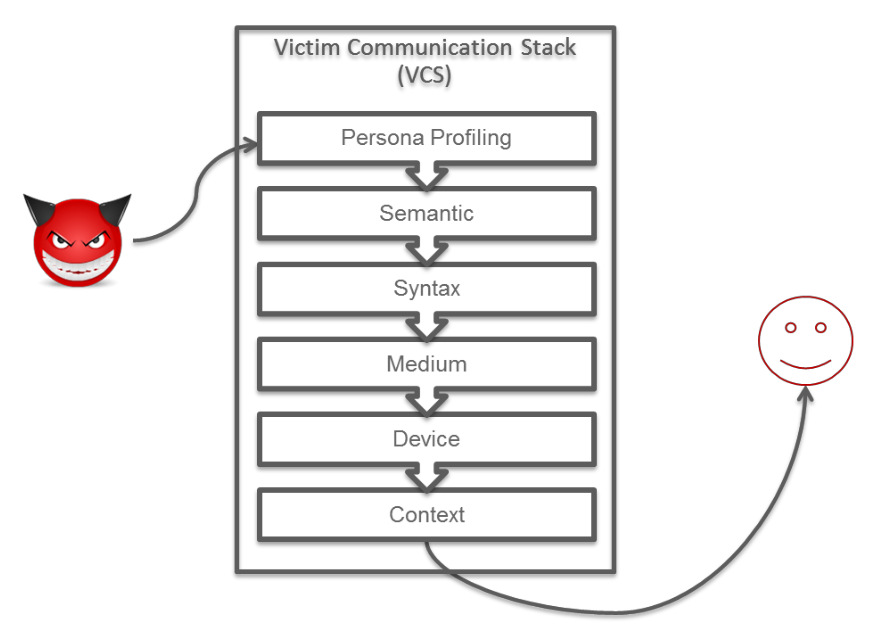
\includegraphics[scale= .25]{VSC.jpg}}
\caption{Social Engineering Phases \cite{Frumento:2017:VCS:3098954.3103156} }
\label{fig}
\end{figure}

\subsection{Habits}
What makes social media such a goldmine for social engineers are the human factors that build the foundation for social media habits.  If every person was to truly keep security and privacy at the forefront of their mind when they were conducting their social media business, then the risk of being compromised would drop significantly.  Completely removing the risk is impossible as 100\% security is an unachievable goal\cite{6320436}. There is a tendency among many information security practitioners to ignore the human factors related to managing social media platforms\cite{6320436}. Organizations put policies in place that dictate the basic usage of social media by an employee, but they don't go into detail about the behavioral factors relate to social media usage.  An organization's social media security culture is dynamic and in constant flux\cite{6320436}.  In order for an organization's social media security culture to be effective, the organization needs to take a holistic approach, which includes understanding and evaluating the human factors related to social media usage. In addition to undestanding the human factors realted to social media usage, an organization needs to have a social media culture that is properly managed with using a clearly defined social media culture managment process as show below in figure 4.   In addition to a social media culture managment process, there needs to be a mechanism in place to support the managment process.  Oehri and Teufel recommend using the Social Media Cluture ASsessment and Reporting Tool (SCART)\cite{teufel}.  
\begin{figure}[htbp]
\centerline{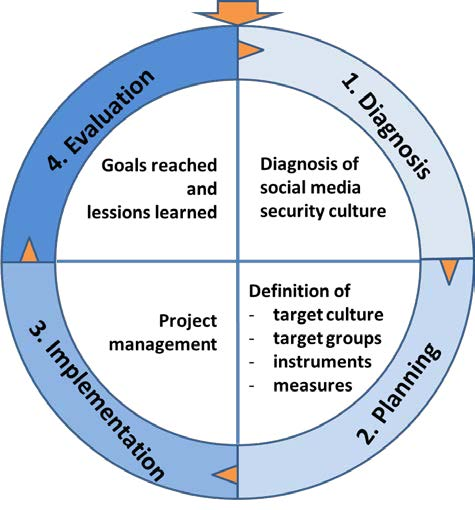
\includegraphics[scale= .75]{SMSC}}
\caption{Social Engineering Phases \cite{6320436} }
\label{fig}
\end{figure}
As previously mentioned, Sheng et al, conducted a study to determine if there was any truth to demographics having anything to do with a person's susceptibility. As was previously noted, Sheng et al determined that demographics didn't really have much to do with susceptibility, although their initial results gave the impression that gender and age may have some impact.  However, Sheng et al did notice that an individual with a higher education was less susceptible than someone who had less of an education. Sheng et al's research implies that if we can better educate individuals, then their susceptibility goes down.  Although this might be true to a certain level, it must be noted that person's behavior and habits will often times come back to circumvent any training that they might have had.  For example, if a person lived in New Hampshire their entire lives, where seatbelts are only required for someone under the age of 18, and this individual moved to Vermont, where everyone is required to wear their seatbelt and there is an avid “click it or ticket” campaign, one would think that the new Vermont resident would adopt begin wearing their seatbelt all the time.  Unfortunately, this is not the case because the habit of not wearing the seatbelt was so significant in their lives prior to moving to Vermont, the operator is more likely to be lackadaisical about wearing the seatbelt. The CDC reported that in 2016 only 84\% of motorists in Vermont wore their seatbelt as directed\cite{CDC}.   Although the seatbelt analogy doesn’t directly apply to social engineering, the idea that a person’s bad habits can’t be changed that easily does. 


 \section{Conclusion}
In this survey, we have looked at how social engineering works and how easy it is for a social engineer to conduct an effective attack against either an individual or an organization.  We have further looked at how social media has become an avenue that social engineers prefer when planning their attacks.  Finally, we looked at how the human factors of susceptibility and habit play a role successful social engineering attacks. 
Social engineering is obviously a serious threat to any user and any organization that uses networked resources. Add to this threat the freely available information that can be found on social media sites, along with the human susceptibility factors that the end user brings to the table, and we have recipe for disaster.  The means the ways we try and combat social engineering has not been able to keep up with the complexity of the attacks that are occurring. More research needs to be conducted in determining the human factors related to a user being susceptible to social engineering, as well as, more research into how we lock down the waterfall of data called social media. Until more research is conducted in these areas, it looks as though the social engineers will continue to win.

\nocite{*}
\bibliographystyle{ieeetran}
\bibliography{Bibliography1}

\end{document}
